%!TEX root = ../thesis.tex

\cleardoublepage
\chapter{Example of Custom GTP Header Format}
\label{appendix:gtp}

This appendix contains a screenshot of a packet captured during normal operation of the WAN Connector (figure \ref{fig:wshark}), displayed using wireshark. The packet dissection shows the use of the GTP hedaer, along with the additional custom header, which is 8 bytes long. The custom header consists of 2 bytes of regular overhead from the GTP protocol as well as a 4 byte timestamp and 2 spare bytes. This packet was captured during regular operation of the WAN Connector, in the jitter experiment.

\begin{figure}[ht]
    \centering
	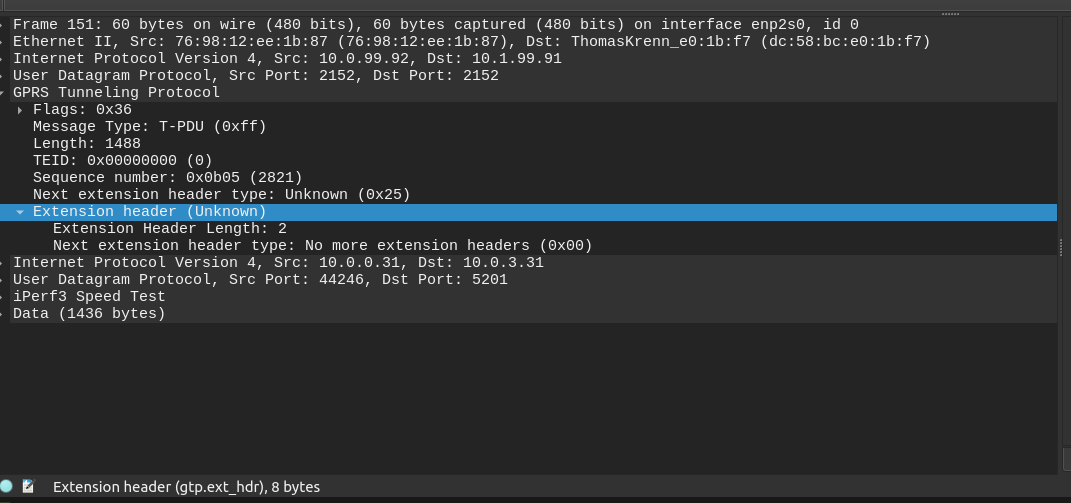
\includegraphics[width=\linewidth]{fig/gtp_2.png}
	\caption{Screenshot of Wireshark Dissection}
	\label{fig:wshark}
\end{figure} 

%
%
%%!TEX root = ../thesis.tex
%
%\cleardoublepage
%\chapter{Selected Parameters from the Simulation}
%\label{appendix:scne}
%
%Here is included a selection of the relevant simulation parameters. These simulation parameters were used to control the SCNE emulation, which generated the data that was adapted to the testbed.
%
%\clearpage
%
%\begin{lstlisting}
%
%default ns3::ScneApplicationHelper::ApplicationIdentifierLevel "CONNECTION"
%default ns3::ScneApplicationHelper::TrafficDirection "BOTH"
%default ns3::ScneApplicationHelper::FwdTrafficModel "CBR"
%default ns3::ScneApplicationHelper::RtnTrafficModel "CBR"
%default ns3::ScneApplicationHelper::FwdTransportLayerProtocol "UDP"
%default ns3::ScneApplicationHelper::RtnTransportLayerProtocol "UDP"
%default ns3::ScneChannelHelper::IslChannelPacketForwardingMode "SINGLE_DESTINATION"
%default ns3::ScneChannelHelper::FwdUserChannelPacketForwardingMode "SINGLE_DESTINATION"
%default ns3::ScneChannelHelper::FwdFeederChannelPacketForwardingMode "SINGLE_DESTINATION"
%default ns3::ScneChannelHelper::RtnUserChannelPacketForwardingMode "SINGLE_DESTINATION"
%default ns3::ScneChannelHelper::RtnFeederChannelPacketForwardingMode "SINGLE_DESTINATION"
%default ns3::ScneGwDeviceHelper::GwFeederDataTransferRate "1000"
%default ns3::ScneGwUserArrivalHelper::DataRate "1Gbps"
%default ns3::ScneGwUserArrivalHelper::Delay "+1ns"
%default ns3::ScneSatDeviceHelper::SatFeederDataTransferRate "1000"
%default ns3::ScneSatDeviceHelper::SatUserDataTransferRate "1000"
%default ns3::ScneSatDeviceHelper::IslDataTransferRate "1000"
%default ns3::ScneSatDeviceHelper::EnableSatUserForcedSingleBeam "false"
%default ns3::ScneSatDeviceHelper::EnableSatFeederPacketErrorRateOverride "false"
%default ns3::ScneSatDeviceHelper::EnableSatUserPacketErrorRateOverride "false"
%default ns3::ScneSatDeviceHelper::EnableIslPacketErrorRateOverride "false"
%default ns3::ScneSatDeviceHelper::SatFeederPacketErrorRate "0"
%default ns3::ScneSatDeviceHelper::SatUserPacketErrorRate "0"
%default ns3::ScneSatDeviceHelper::IslPacketErrorRate "0"
%default ns3::ScneSimulationHelper::RoutingProtocol "GLOBAL"
%default ns3::ScneSimulationHelper::MobilityModel "TRACE"
%default ns3::ScneSimulationHelper::EnableDataPackageValidation "false"
%default ns3::ScneSimulationHelper::EnableConcatenatedInputData "false"
%default ns3::ScneSimulationHelper::EnableGlobalRoutingMultipleRootExitFiltering "true"
%default ns3::ScneSimulationHelper::EnableGlobalRoutingIslIpFiltering "true"
%default ns3::ScneSimulationHelper::Mtu "1500"
%default ns3::ScneUtDeviceHelper::UtUserDataTransferRate "1000"
%default ns3::ScneUtDeviceHelper::EnableUtUserPacketErrorRateOverride "false"
%default ns3::ScneUtDeviceHelper::UtUserPacketErrorRate "0"
%default ns3::ScneUtUserArrivalHelper::DataRate "1Gbps"
%default ns3::ScneUtUserArrivalHelper::Delay "+1ns"
%default ns3::ScneAccessController::MinimumValidCarrierPowerInDbw "-500"
%default ns3::ScneIpv4GlobalRouting::RandomEcmpRouting "false"
%default ns3::ScneIpv4GlobalRouting::RespondToInterfaceEvents "false"
%default ns3::ScneIpv4L3Protocol::DefaultTtl "64"
%default ns3::ScneIpv4L3Protocol::FragmentExpirationTimeout "+3e+10ns"
%default ns3::ScneIpv4L3Protocol::EnableDuplicatePacketDetection "false"
%default ns3::ScneIpv4L3Protocol::DuplicateExpire "+1e+06ns"
%default ns3::ScneIpv4L3Protocol::PurgeExpiredPeriod "+1e+09ns"
%default ns3::ScneTxScheduler::MaximumBufferSize "10"
%default ns3::ScneStats::EnableApplicationDelayStats "true"
%default ns3::ScneStats::EnablePerNodeApplicationDelayStats "true"
%default ns3::ScneStats::EnableApplicationPacketLossRateStats "true"
%default ns3::ScneStats::EnablePacketDropStats "true"
%default ns3::ScneStats::EnablePacketDelayTrace "true"
%default ns3::ScneStats::PeriodicThroughputBinWidth "0.001"
%default ns3::ScneStats::PacketDelayBinWidth "1e-06"
%default ns3::ScneStats::TracingStartTime "+0ns"
%default ns3::ScneStats::TracingStopTime "+8.64e+13ns"
%default ns3::ScneStats::DeviceTxLoadTraceInterval "+6e+10ns"
%default ns3::ScneStats::PositionTraceInterval "+6e+10ns"
%default ns3::ScneStats::DeviceTxBufferTraceInterval "+6e+10ns"
%default ns3::ScneStats::GwUserNodeTraceMode "TRACE_ALL"
%default ns3::ScneStats::GwUserNodeSelectionToTrace ""
%default ns3::ScneStats::UtUserNodeTraceMode "TRACE_ALL"
%default ns3::ScneStats::UtUserNodeSelectionToTrace ""
%default ns3::ScneStatsPacketHandler::PeriodicBitrateStep "+5e+09ns"
%default ns3::ScneStatsPacketHandler::PeriodicBitrateWindowLength "+1e+10ns"
%default ns3::ScneStatsPacketHandler::PeriodicBitrateWindowSize "4294967295"
%default ns3::ScneAdvancedOnOffApplication::PacketInterval "ns3::ConstantRandomVariable[Constant=0.008]"
%default ns3::ScneAdvancedOnOffApplication::PacketSize "ns3::ConstantRandomVariable[Constant=512]"
%default ns3::ScneAdvancedOnOffApplication::EnableConstantBursts "true"
%default ns3::ScneAdvancedOnOffApplication::StartInOffState "true"
%default ns3::ScneAdvancedOnOffApplication::MaxBytes "0"
%default ns3::ScneCbrApplication::PacketSize "1400"
%default ns3::ScneCbrApplication::Interval "+1e+10ns"
%
% 
%\end{lstlisting} 
